\section{Redes Neuronais Artificiais}\label{sec:ArtificialNeuralNetwork}

 
As redes neuronais artificiais foram inspiradas no sistema biológico de redes neuronais constituintes do cérebro.
Estes sistemas foram implementados para executar tarefas através de exemplos anteriores (casos de teste), não sendo assim necessário programação específica para o efeito. Por exemplo, estes sistemas são capazes de identificar um certo objeto numa imagem, este processo passa por treinar o sistema com imagens, as quais foram previamente identificadas como tendo ou não o objeto. Usando estes casos de teste o sistema é capaz de encontrar as mesmas características noutras imagens e assim sendo identificar se o objeto está ou não presente na imagem.
Como funciona
 
Uma rede neuronal artificial, à semelhança das redes neuronais, é representada por um conjunto de neurónios, unidos uns aos outros através de sinapses para transmitir informação entre eles.
Os neurónios podem apresentar um estado (normalmente representado por um número real entre 0 e 1) e podem também, à semelhança das sinapses, ter um “peso”, que consiste num valor que varia ao longo do processo de aprendizagem de forma a obter resultados mais coerentes. Além disto, podem também apresentar um patamar, tal que, apenas os sinais acima ( ou abaixo) do mesmo são reenviados para o próximo neurónio.
Por norma os neurónios estão organizados por camadas. Diferentes camadas tem objetivos diferentes,podendo-se separar os neurónios em 3 tipos, neurónios de entrada (input do programa), neurónios intermediários e neurónios de saída (output).

Neste momento as redes neuronais já se encontram presentes no nosso dia a dia e conseguem desempenhar tarefas tais como, reconhecimento de imagens e fala, tradução de conteúdos ou aplicações ao nível de redes sociais e plataformas de comércio eletrónico.

\begin{figure}[H]
    \centering
    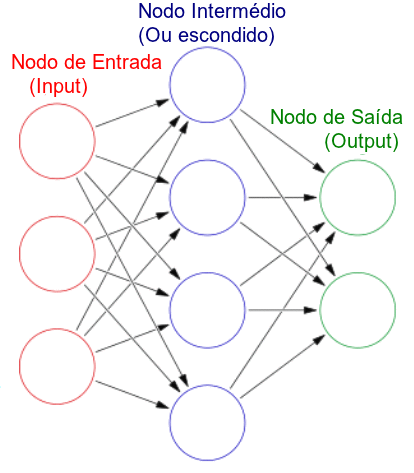
\includegraphics[scale=0.3]{img/ann1.png}
    \caption{Exemplo de uma rede neuronal}
    \label{fig:Rede Neuronal}
\end{figure}

\subsection{Componentes das redes}

Uma rede neuronal artificial é comparável a um grafo, onde os nodos correspondem a neurónios e as sinapses correspondem às ligações ou arestas. Para que estes grafos funcionem são necessários os seguintes componentes:

\begin{enumerate}  
\item Neurônios
\item Um neurônio de uma rede artificial é constituído por:
\item Um parâmetro de ativação segundo um tempo discreto;
\item Um patamar, que pode apenas ser alterado pela função de aprendizagem;
\item Uma função de ativação que permite uma nova ativação num novo tempo;
\item Uma função de output, que forma o output da ativação. \ldots 
\end{enumerate}
 
Um neurónio de input não tem predecessor, serve como interface da rede e é usado para alimentar a rede com nova informação, analogamente, os neurónios de saída não possuem sucessor, e servem como output da rede.
Função de Aprendizagem
A função de aprendizagem é um algoritmo que modifica a rede neuronal ao longo do seu treino de forma a obter melhores resultados, modificando o peso e patamar dos neurónios e sinapses dentro da rede.
Sinapses
Nas redes neuronais, os neurónios são unificados por ligações as quais chamamos sinapses, estas têm um peso que vai sendo alterado à medida que a aprendizagem ocorre, sempre com o objetivo de melhorar a capacidade de previsão da rede.
Função de custo
Esta função é usada para avaliar a função de aprendizagem, sendo que, quanto melhor a função de aprendizagem, menor será o custo desta.
 
\subsection{Aprendizagem}

As redes neuronais atraíram interesse devido a sua capacidade de aprendizagem. 
No meio de redes neuronais, aprendizagem significa, dada uma tarefa e um conjunto de funções, usar um conjunto de observações (casos de teste) para encontrar a função que melhor resolve o problema.
Um dos conceitos mais importantes na aprendizagem é a função de custo, que mede quão longe está a solução atual dos resultados pretendidos. Através do output desta função, o algoritmo de aprendizagem procura no conjunto de funções a função que melhor resolve o problema ( função com menor custo).
A função de custo é escolhida consoante o problema apresentado.
